\chapter{Unsupervised Learning}
Up to this point, our learning paradigm was of \textbf{supervised batch learning}. Given a sample space $\Xc$ and a label/response space $\Yc$, we were interested in \textbf{prediction}: finding some way to predict $y\in\Yc$ corresponding to a new unseen sample $x\in\Xc$, based on a training set of labeled samples $\trainset$. However, there are many learning problems that do not fit into this framework of supervised batch learning. In one such set of problems we still consider a domain set $\Xc$ but there is no label/response space. Namely, the data is of the form $S=\left\{\x_i\right\}^m_{i=1}$ where $\x_i\in\Xc$. Such problems are called \textbf{un-supervised} learning problems, and the goal is to infer different properties of $\Xc$. A few examples are:\\
\begin{itemize}
\item \textbf{Uncovering low-dimensional structures:} In some cases we have reason to believe that some given data, though represented in high dimension, could actually be represented in a lower dimension. Consider for example the MNIST database of handwritten digits. This coprus of $28$-by-$28$ pixels grey-scaled images shows scans of people handwriting of the digits $0,\ldots,9$. Though each imange (sample) is represented in $\R^{28\times 28}$, there are very few variations on how people write digits. In \autoref{pca_data_example} we can see that in most images a big area in the surrounding of the image remains constant. This means that these pixels are not informative for predicting the digit. In addition, even though two images of the same digit (for example the digit $3$ as seen below) show differences, they are still mostly the same. Therefore, it might be possible to \textbf{reduce the dimension} of the samples into a more compact, of lower dimension, representation.

\begin{figure}[h!]
	\centering
	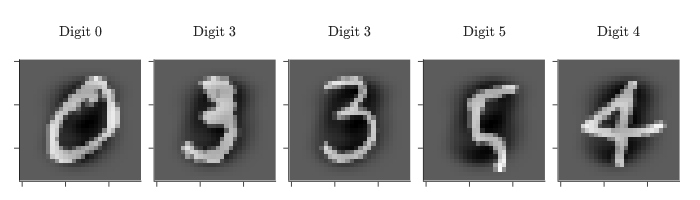
\includegraphics[width=0.7\textwidth]{chapters/unsupervised.learning/figures/pca_data_Digit.png}
	\caption{\textbf{MNIST Digits Dataset}: A set of 5 labelled samples from the MNIST Digits dataset}\label{pca_data_example}
\end{figure}

~\\
\item \textbf{Clustering:} Often, when we are given a dataset, we are interested in grouping (or segmenting) it into subsets such that those samples within each cluster are in some way more "closely related" to each other than to samples in other subsets. We refer to these subsets as \textit{clusters}. Consider once more the MNIST digits dataset. In general, it seems logical that images of the same digit resemble each other more than images of different digits. If we would to try to cluster it (that is, segment its samples into different subsets) we would hope to get 10 separate subsets, each containing images of a specific digit.\\
\item \textbf{Anomaly detection:} Suppose we are interesting in detecting when some given system is not behaving "as usual". Consider an air conditioning system or power plant. We place sensors in the system and would like to get a warning when something is behaving "strange". We do not know what exactly a "strange" behavior would look like, but it might be caused due to some mechanical malfunction, a software problem or even a cyber attack. We monitor the state of the system at all times. If we have installed $d$ sensors, each time we take a reading of the system we get a sample $\x_i\in\R^d$. We train out learning system on the readings $\x_1,\ldots,\x_m\in\R^d$ where we believe these represent the normal state of the system. Now, given a new reading $\x\in\R^d$, is it "normal"? or is there something wrong? We are required to make a decision without have seeing the system in the "wrong"/"abnormal"/"strange" state before.
\end{itemize}

~\\\autoref{unsupervised_img} shows an example of performing both clustering and dimensionality reduction. In the figure we visualize a dataset of single-cell RNA-sequencing gene expression. This dataset consists of 8850 cells (samples, seen in figure as the individual dots) over 30449 genes (features) where for each cell we have the level of expression (a number in $\N_0$) of the specific gene. The analysis of this dataset included:
\begin{itemize}
	\item \textbf{Dimensionality reduction}: to reduce dimensionality from the original 30449 dimensional features space to a lower 25 dimensional space. Further computations were performed over this lower dimension space, making computations simpler. The dimensionaliy reduction algorithm in use is the PCA algorithm which we discuss below (\autoref{pca}).\\
	\item \textbf{Clustering}: Over the reduced, 25 dimensional, feature space a clustering algorithm was used. This algorithm split the dataset into different clusters. These  different clusters are represented using different colors.\\
	\item \textbf{Secondary dimensionality reduction}: To help with visualizing the data, another dimensionality reduction algorithm was used. This time, dimension was reduced to a two dimensinoal space, enabling clear overview of both data and clustering results.
\end{itemize}

\begin{figure}[h!]
	\centering
	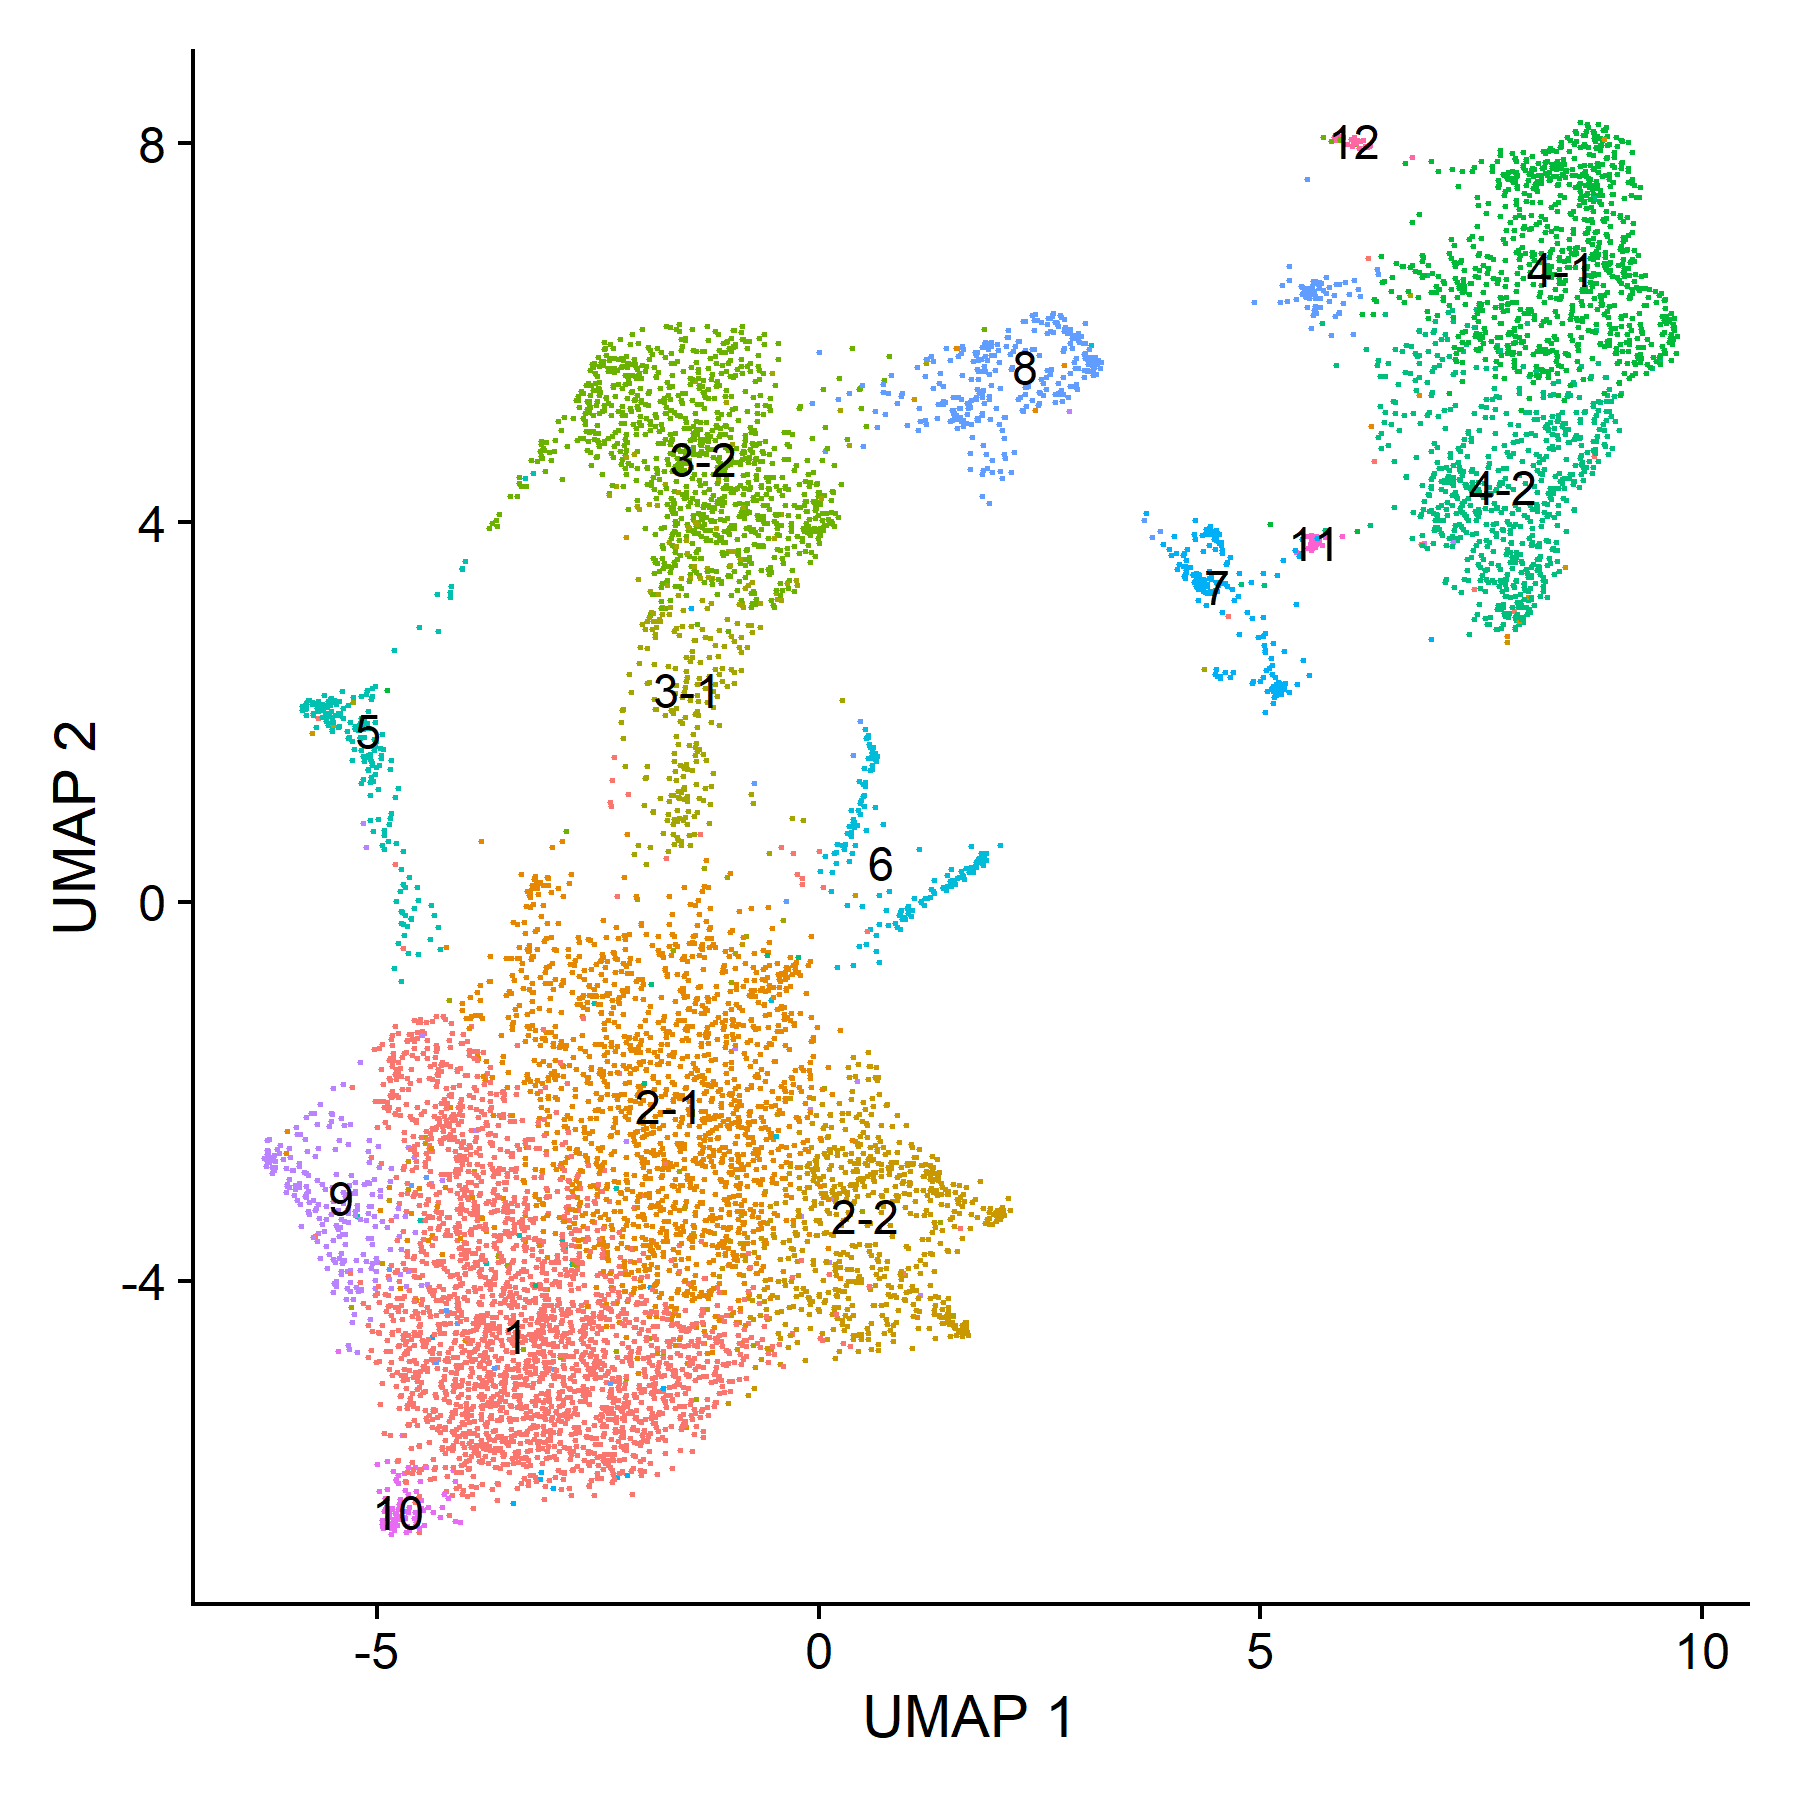
\includegraphics[width=0.5\textwidth]{chapters/unsupervised.learning/figures/single.cell.dim.clust.png}
	\caption{\textbf{Clustering and Dimensionality Reduction}}\label{unsupervised_img}
\end{figure}

\section{Dimensionality Reduction}
Dimensionality reduction is the process of mapping some high dimensional space (the ambient space) to some new low dimensional space (the intrinsic space). Given a dataset $\x_1,\ldots,\x_m\in\R^d$ we want to find some mapping $f:\R^d\rightarrow\R^k$ for $k \ll d$, where $f\left(\x_1\right),\ldots,f\left(\x_m\right)$ still resembles $\x_1,\ldots,\x_m$ in some sense. Different dimensionality reduction techniques are usually separated to linear- and non-linear techniques depending on the selected $f$. 
\\~\\
There are different reasons to study and apply dimension reduction:
\begin{itemize}
	\item \textbf{Learnability:} Some learning algorithms work better when the dimension $d$ is small compared with the training sample size $m$, and might even fail if $d$ is too large. Recall for example the case of linear regression. Though in both cases $m<d$ and $d<m$ we have a closed form solution, we have seen that if $d<m$ the results are numerically unstable. \\
	\item \textbf{Computation:} For many algorithm the time- and space complexity depends on the dimension $d$. By reducing the data dimensionality we can use fewer computational resources to perform the learning task we intended. \\
	\item \textbf{Visualization:}  Visualization is an extremely useful tool both for explaining and exploring our data. If we can reduce dimension to $k\leq 4$ then we can plot the data (possibly on a 3 dimensional axis, with the forth dimension represented by color).
\end{itemize}


\subsection{Principal Component Analysis (PCA)}\label{pca}
Let $\x_1,\ldots,\x_m\in\R^d$ be some dataset and suppose that it approximately resides in some lower $k$-dimensional linear subspace of $\R^d$. We would like to find some linear transformation of the data to project it on that lower dimension subspace. To do so we need to solve two challenges:
\begin{enumerate}
	\item There are infinitely many subspaces we could consider. Which subspace should we choose and how should we acquire it?\\
	\item Even if we knew the subspace, projecting the data-points $\x\in\R^d$ onto the subspace does not yet reduce the dimension. We would want to find a way to represent each sample by the $k$ coordinates of that sample \textit{in} the subspace. This is also known as the \textit{embedding} of the samples.
\end{enumerate}~\\

In the case of Principal Component Analysis (PCA), given a dataset $\x_1,\ldots,\x_m\in\R^d$ we are searching for some linear transformation such that we minimize the squared error between the original samples and their transformation:
\begin{equation}
f^*\coloneqq\underset{f}{argmin} \sum^m_{i=1}\norm{\x_i - f\left(\x_i\right)}^2
\end{equation}
This problem can be formulated in four different ways:
\begin{enumerate}
	\item Finding the closest affine subspace to the points.
	\item Finding the affine subspace that retains most of the variation seen in the data (sometimes referred to as \textit{signal}).
	\item Finding the affine subspace that minimizes the distortion of the pairwise distances between points in the ambient- compared to the intrinsic spaces.
	\item Generalization of linear regression with Gaussian noise both in the explanatory variables directions and in the response direction. This interpretation is also known as probabilistic PCA.
\end{enumerate}~\\
Here, we will discuss the first two, most common, formulations.

\subsubsection{Closest Affine Subspace}
To simply the problem of finding the closest affine subspace, let us assume that the data is centered around the origin and as such instead of searching for some affine subspace, we are searching for an "ordinary" subspace. Therefore, we are searching for some linear map $W:\R^d\rightarrow\R^k$ and an "inverse" linear map $U:\R^k\rightarrow\R^d$
\begin{equation}
W^*,U^* = \underset{W\in\R^{d\times k},U\in\R^{k\times d}}{argmin} \sum_{i=1}^m \norm{\x_i-UW\x_i}^2
\label{eqn:pca1}
\end{equation}


\begin{lemma}
Let $\left(U,W\right)$ be a solution to (\ref{eqn:pca1}). Then $U$'s columns are orthonormal and $W=U^\top$.
\end{lemma}
\begin{proof}
Let $U,W$ be some matrices and consider the mapping $\x\mapsto \left(UW\right)\x$. The matrix $\left(UW\right)$ is a $d$-by-$d$ matrix of rank $k$, whos image is a $k$ dimensional subspace of $\R^d$. Denote $S\coloneqq Im\left(UW\right)$. As $\x\in\R^d$ and $\left(UW\right)\x\in S$, it holds that the projection that minimizes $\norm{\x-UW\x}_2$ is the orthogonal projection onto the subspace. In addition, the point in $S$ closest to $\x$, namely the orgothonal projection pf $\x$ onto $S$, is given by $VV^\top\x$ where the columns of $V$ are an orthonormal basis of $S$:
$$ \forall \vv{u}\in S\quad \norm{\x-\vv{u}}_2 \geq \norm{\x-VV^\top\x}_2 $$
Thus, the solution to \ref{eqn:pca1} is $U$ with orthonormal columns and $W\coloneqq U^\top$. 
\end{proof}

Based on the above lemma, we can now write an equivalent problem to the PCA problem presented in \ref{eqn:pca1}. Observe that:
$$
\begin{array}{ccl}
\norm{\x-UU^\top\x}^2 & = & \norm{\x}^2 -2\x^\top UU^\top\x + \x^\top UU^\top UU^\top\x \\
& = & \norm{\x}^2 -\x^\top UU^\top\x\\
& \overset{\left(*\right)}{=} & \norm{\x}^2 -\left(U^\top\x\right)^\top U^\top\x\\
& = & \norm{\x}^2 - trace\left(U^\top\x \left(U^\top\x\right)^\top\right) \\
& = & \norm{\x}^2 - trace\left(U^\top\x\x^\top U\right)
\end{array}$$

where $\left(*\right)$ is because $\forall \vv{v},\vv{u}\in\R^k \,\, trace\left(\vv{u}\vv{v}^\top\right)=\vv{v}^\top\vv{u}$. As the trace is a linear operator we can re-write an equivalent problem:
\begin{equation}
U^* = \underset{U\in\R^{d\times k},U^\top U=I}{argmax} \sum_{i=1}^m trace\left(U^\top\x_i\x_i^\top U\right) = \underset{U\in\R^{d\times k},U^\top U=I}{argmax} trace\left(U^\top\sum_{i=1}^m \x_i\x_i^\top U\right)
\label{eqn:pca2}
\end{equation}



\begin{theorem}\label{pca_closest_subspace}
Let $A=\sum\x_i\x_i^\top$ and let $\vv{u}_1,\ldots,\vv{u}_k$ be the $k$ leading eigenvectors of $A$. Then, the solution to the PCA problem is given by $U\in\R^{d\times k}$ whose columns are $\vv{u}_1,\ldots,\vv{u}_k$.
\end{theorem}
\begin{proof}
Denote $A=\sum\x_i\x_i^\top$. Then, we need to solve $$ \underset{U\in\R^{d\times k},U^\top U=I}{argmax} trace\left(U^\top A U\right)$$
Notice that $A$ is a square symmetric matrix so let $A=VDV^\top$ be the EVD of $A$, where the diagonal of $D$ are the eigenvalues of $A$ in decreasing order $\lambda_1\geq \ldots \geq \lambda_d$ and the columns of $V$ are the corresponding eigenvectors. So:
$$
\begin{array}{cclcl}
trace\left(U^\top AU\right) & = & trace\left(U^\top V D V^\top U\right) & \overset{\left(*\right)}{=} & trace\left(B^\top D B\right)\\
& = & trace\left(DBB^\top\right) &=& \sum_{j=1}^d\left[DBB^\top\right]_{jj} \\
& = & \sum_{j=1}^d \left[D\right]_{j} \left[BB^\top\right]_{\cdot,j} & = & \sum_{j=1}^d \lambda_j\cdot \left[BB^\top\right]_{jj} \\
& = & \sum_{j=1}^d \lambda_j\cdot \sum_{i=1}^k B_{ji}^2
\end{array}
$$
where $B=V^\top U\in \R^{d\times k}$. Notice that 
$$
\begin{array}{c}
B^\top B=U^\top VV^\top U = I_d\\
\Downarrow\\
\indc{j\neq i} = \inprod{\left[B^\top\right]_j}{\left[B\right]_{\cdot,i}} = \inprod{\left[B\right]_{\cdot,j}}{\left[B\right]_{\cdot,i}}
\end{array}$$
meaning that the columns of $B$ are orthonormal, and therefore $\sum_{j=1}^d\sum_{i=1}^k B_{ji}^2 = k$. Based on $B$, define $\widetilde{B}=\left[\begin{array}{c|c} B & M\end{array}\right] \in \R^{d \times d}$ with $M\in\R^{d\times \left(d-k\right)}$ completing an orthonormal basis in $R^d$. If so, then $\forall j\,\, \sum_{i=1}^d\widetilde{B}^2_{ji}=1$, which implies that $\sum_{i=1}^k B_{ji}^2$. As such 
$$ trace\left(U^\top A U\right) = \sum_{j=1}^d \lambda_j\cdot \sum_{i=1}^k B_{ji}^2 \leq \underset{\beta\in \left[0,1\right]^d, \norm{\beta}_1\leq k}{max} \sum_{j=1}^d \lambda_j \beta_j =\sum_{j=1}^k \lambda_k$$

To conclude the proof, let $U$ be the matrix whose columns are the $k$ leading eigenvalues of $A$ then $$
U^{\top}AU=\left[\begin{array}{c}
u_{1}^{\top}\\
\vdots\\
u_{k}^{\top}
\end{array}\right]A\left[\begin{array}{ccc}
u_{1} & \cdots & u_{k}\end{array}\right]=\left[\begin{array}{c}
u_{1}^{\top}\\
\vdots\\
u_{k}^{\top}
\end{array}\right]\left[\lambda_{1}\begin{array}{ccc}
u_{1} & \cdots & \lambda_{k}u_{k}\end{array}\right]=diag\left(\lambda_{1},\ldots,\lambda_{k},\overset{d-k}{\overbrace{0,\ldots,0}}\right)
$$
and $trace\left(U^\top A U\right) = trace\left(diag\left(\lambda_{1},\ldots,\lambda_{k},0,\ldots,0\right)\right)=\sum^k \lambda_i$, as requested.
\end{proof}


~\\\paragraph{Generalizing for affine subspaces:} In the above theorem we in-fact found the closest subspace- and not the closest affine subspace to the data. To find the closest affine subspace, we would like to allow the mapping $W$ to be \textbf{affine}. To achieve this we generalize the above by considering $W:\R^d\rightarrow\R^k$ to be of the form $$ W\left(\x\right)\coloneqq\widetilde{W}\left(\x-\mu\right),\quad \mu\in\R^d,\, \widetilde{W}:\R^d\rightarrow\R^k$$ 
This allows us to ``shift`` the data before applying the linear map $\widetilde{W}$. When adding $\mu$ to the optimization problem above, we find that the minimizer $\mu$ is given by: $ \mu = \frac{1}{m}\sum \x_i $. This is the empirical mean of the data, often denoted by $\overline{\x}$. So, in order to find the closest affine subspace to the data we center the matrix $A$: $$ A\coloneqq \sum_{i=1}^m \left(\x_i -\overline{\x}\right)\left(\x_i -\overline{\x}\right)^\top $$

yielding the following pseudo-code for the PCA algorithm:

\begin{algorithm}
	\caption{PCA}\label{pca_pseudo}
	\begin{algorithmic}
		\Procedure{PCA}{$\X$, $k$}\Comment{$\X$ The design matrix of $m$ samples and $d$ features}
		\State Compute $A\gets \sum_{i=1}^m \left(\x_i-\overline{\x}\right)\left(\x_i-\overline{\x}\right)^\top$ 
		\State Let $\vv{u}_1,\ldots,\vv{u}_k$ be the eigenvectors of $A$ corresponding the largest eigenvalues.
		\State \textbf{return} $\vv{u}_1,\ldots,\vv{u}_k$
		\EndProcedure
	\end{algorithmic}
\end{algorithm}

~\\ The eigenvalues of $A$, $\lambda_1\geq\ldots\geq\lambda_d$ are referred to as the \textbf{Principal Values} of $\X$. The eigenvectors of $A$, $\vv{u}_1,\ldots,\vv{u}_d$ are referred to as the \textbf{Principal Components}. Notice that the matrix $A$ is a $d$-by-$d$ positive semi-definite matrix. Therefore the PCA algorithm is in fact a case of a matrix diagonalization algorithm where we simply try to find the eigenvalues and eigenvectors of some target matrix.


\subsubsection{Maximum Retained Variance}
Another way to think about PCA is as a dimensionality reduction technique that maintains the maximum amount of variance of the data possible in a $k<d$ dimensional subspace. To prove so we will have to solve a constraint maximization problem using Lagrange Multipliers. 

\todo{Explain lagrange multipliers}

\begin{theorem}\label{pca_max_var}
Let $\X$ be an $m$-by-$d$ design matrix. The projection of $\X$ onto a $k$ dimensional linear subspace that retains maximum of the variance in $\X$ is given by the matrix $U\in\R^{d\times k}$ whose columns are the $k$ eigenvectors with leading eigenvalues of the sample covariance matrix $S$.
\end{theorem}
\begin{proof}
We begin with considering the projection onto a one-dimensional subspace. Without loss of generality let $\vv{v}\in\R^d$ be a unit vector used to project the data onto. The variance of the projection of each $\x_i$ onto $\vv{v}$, $\vv{v}^\top\x_i$ is given by:
$$
\begin{array}{rclcl}
	\E\left[\vv{v}^\top \x\right] & = & \frac{1}{m}\sum \vv{v}^\top \x_i =\vv{v}^\top \overline{\x} \\
	\\
	Var\left(\vv{v}^\top \x\right) & = & \E_{\x}\left[\left(\vv{v}^\top \x_i - \E_{\x}\left[\vv{v}^\top \x\right]\right)^2\right]
	& = & \frac{1}{m}\sum\left(\vv{v}^\top \x_i - \vv{v}^\top \overline{\x}\right)^2 \\
	& = & \frac{1}{m}\sum\left[\vv{v}^\top\left(\x_i - \overline{\x}\right)\right]^2
	& = & \frac{1}{m}\sum \left[\vv{v}^\top\left(\x_i - \overline{\x}\right)\right]\left[\vv{v}^\top\left(\x_i - \overline{\x}\right)\right]^\top \\
	& = & \frac{1}{m}\sum \vv{v}^\top\left(\x_i - \overline{\x}\right)\left(\x_i - \overline{\x}\right)^\top \vv{v}
	& = & \vv{v}^\top\left[\frac{1}{m}\sum\left(\x_i - \overline{\x}\right)\left(\x_i - \overline{\x}\right)^\top\right]\vv{v} \\
	& = & \vv{v}^\top S \vv{v}
\end{array}
$$
So now let us maximize the projected variance with respect to $\vv{v}$:
$$ \widehat{\vv{v}} = \underset{\norm{v}=1}{argmax}\, \vv{v}^\top S\vv{v} $$ To solve this optimization problem we will use the Lagrange multipliers method with the constraint $g\left(\vv{v}\right) = 1-\vv{v}^\top \vv{v}$. So the lagrangian is given by:
$$\begin{array}{c}
\Lc = \vv{v}^\top S \vv{v} + \lambda g\left(\vv{v}\right)\\
\Downarrow\\
\frac{\partial}{\partial \vv{v}}\Lc = 2S\vv{v} - 2\lambda \vv{v} = 0
\end{array}$$
Therefore the maximizer of $\vv{v}^\top\vv{v}$ must be an eigenvector of $S$. Notice that by left-multiplying the derivative by $\vv{v}^\top$ we find that the retained variance itself is given by: $$ \vv{v}^\top S\vv{v} = \lambda\vv{v}^\top\vv{v} \overset{\norm{\vv{v}}=1}{=} \lambda$$
Thus, the maximal retained variance is the largest eigenvalue $\lambda_1$, achieved by $\vv{v}\coloneqq\vv{u}_1$.

~\\Next, let us find the direction that retains the second largest amount of variance. As we are looking for an orthogonal projection we add an additional constraint that this direction is orthogonal to $\vv{u}_1$:

$$ \widehat{\vv{v}} = \underset{\norm{\vv{v}}=1,\, \vv{v}^\top \vv{u}_1 = 0}{argmax}\, \vv{v}^\top S\vv{v} $$

As before, when solving the constraint optimization problem for $\vv{v}$ we find that the direction retaining the second largest amount of variance is $\vv{v}\coloneqq \vv{u}_2$, with the amount of variance being $\lambda_2$. Proving by induction we get that $\forall k\leq d$, the $k$ dimensional subspace that retains maximal variance of projecting $\X$ onto it, is given by the $k$ leading eigenvectors of $S$.
\end{proof}


\subsubsection{Link Between Closest Subspace and Maximum Variance}
In the above we have seen two interpretations of PCA: one as closest subspace and one as maximizing variance. To understand how the two are connected consider the dataset seen in \autoref{pca_interp_link} and specifically the $\x_i$ data-point. Notice that by orthogonally projecting $\x_i$ onto $\vv{u}_1$ a right-angle triangle is formed where:
\begin{itemize}
	\item The edge denoted by $a$ is the size of the projection of $\x_i$ onto $\vv{u}_1$: $a\coloneqq \norm{\x_i^\top \vv{u}_1}$. This is the measure maximized in the maximum variance interpretation.
	\item The edge denoted by $b$ is the distance between the original data-points $\x_i$ and its orthogonal projection onto $\vv{u}_1$: $b\coloneqq \norm{\x_i - \x_i \vv{u}_1}$. This is the measure minimized in the closest subspace interpretation.
	\item The edge denoted by $c$ is the size of $\x_i$: $c\coloneqq \norm{\x_i}$.
\end{itemize}

As this is a right-angle triangle, we know from the Pythagorean theorem that $c^2=a^2+b^2$. Therefore, if we find a PCA solution that minimizes $b$ (the closest subspace), we in fact find a solution that maximizes $a$. Similarly by finding a solution that maximizes $a$ (maximal projected variance), we find a solution that minimizes $b$.

\begin{figure}[!h]
	\centering
	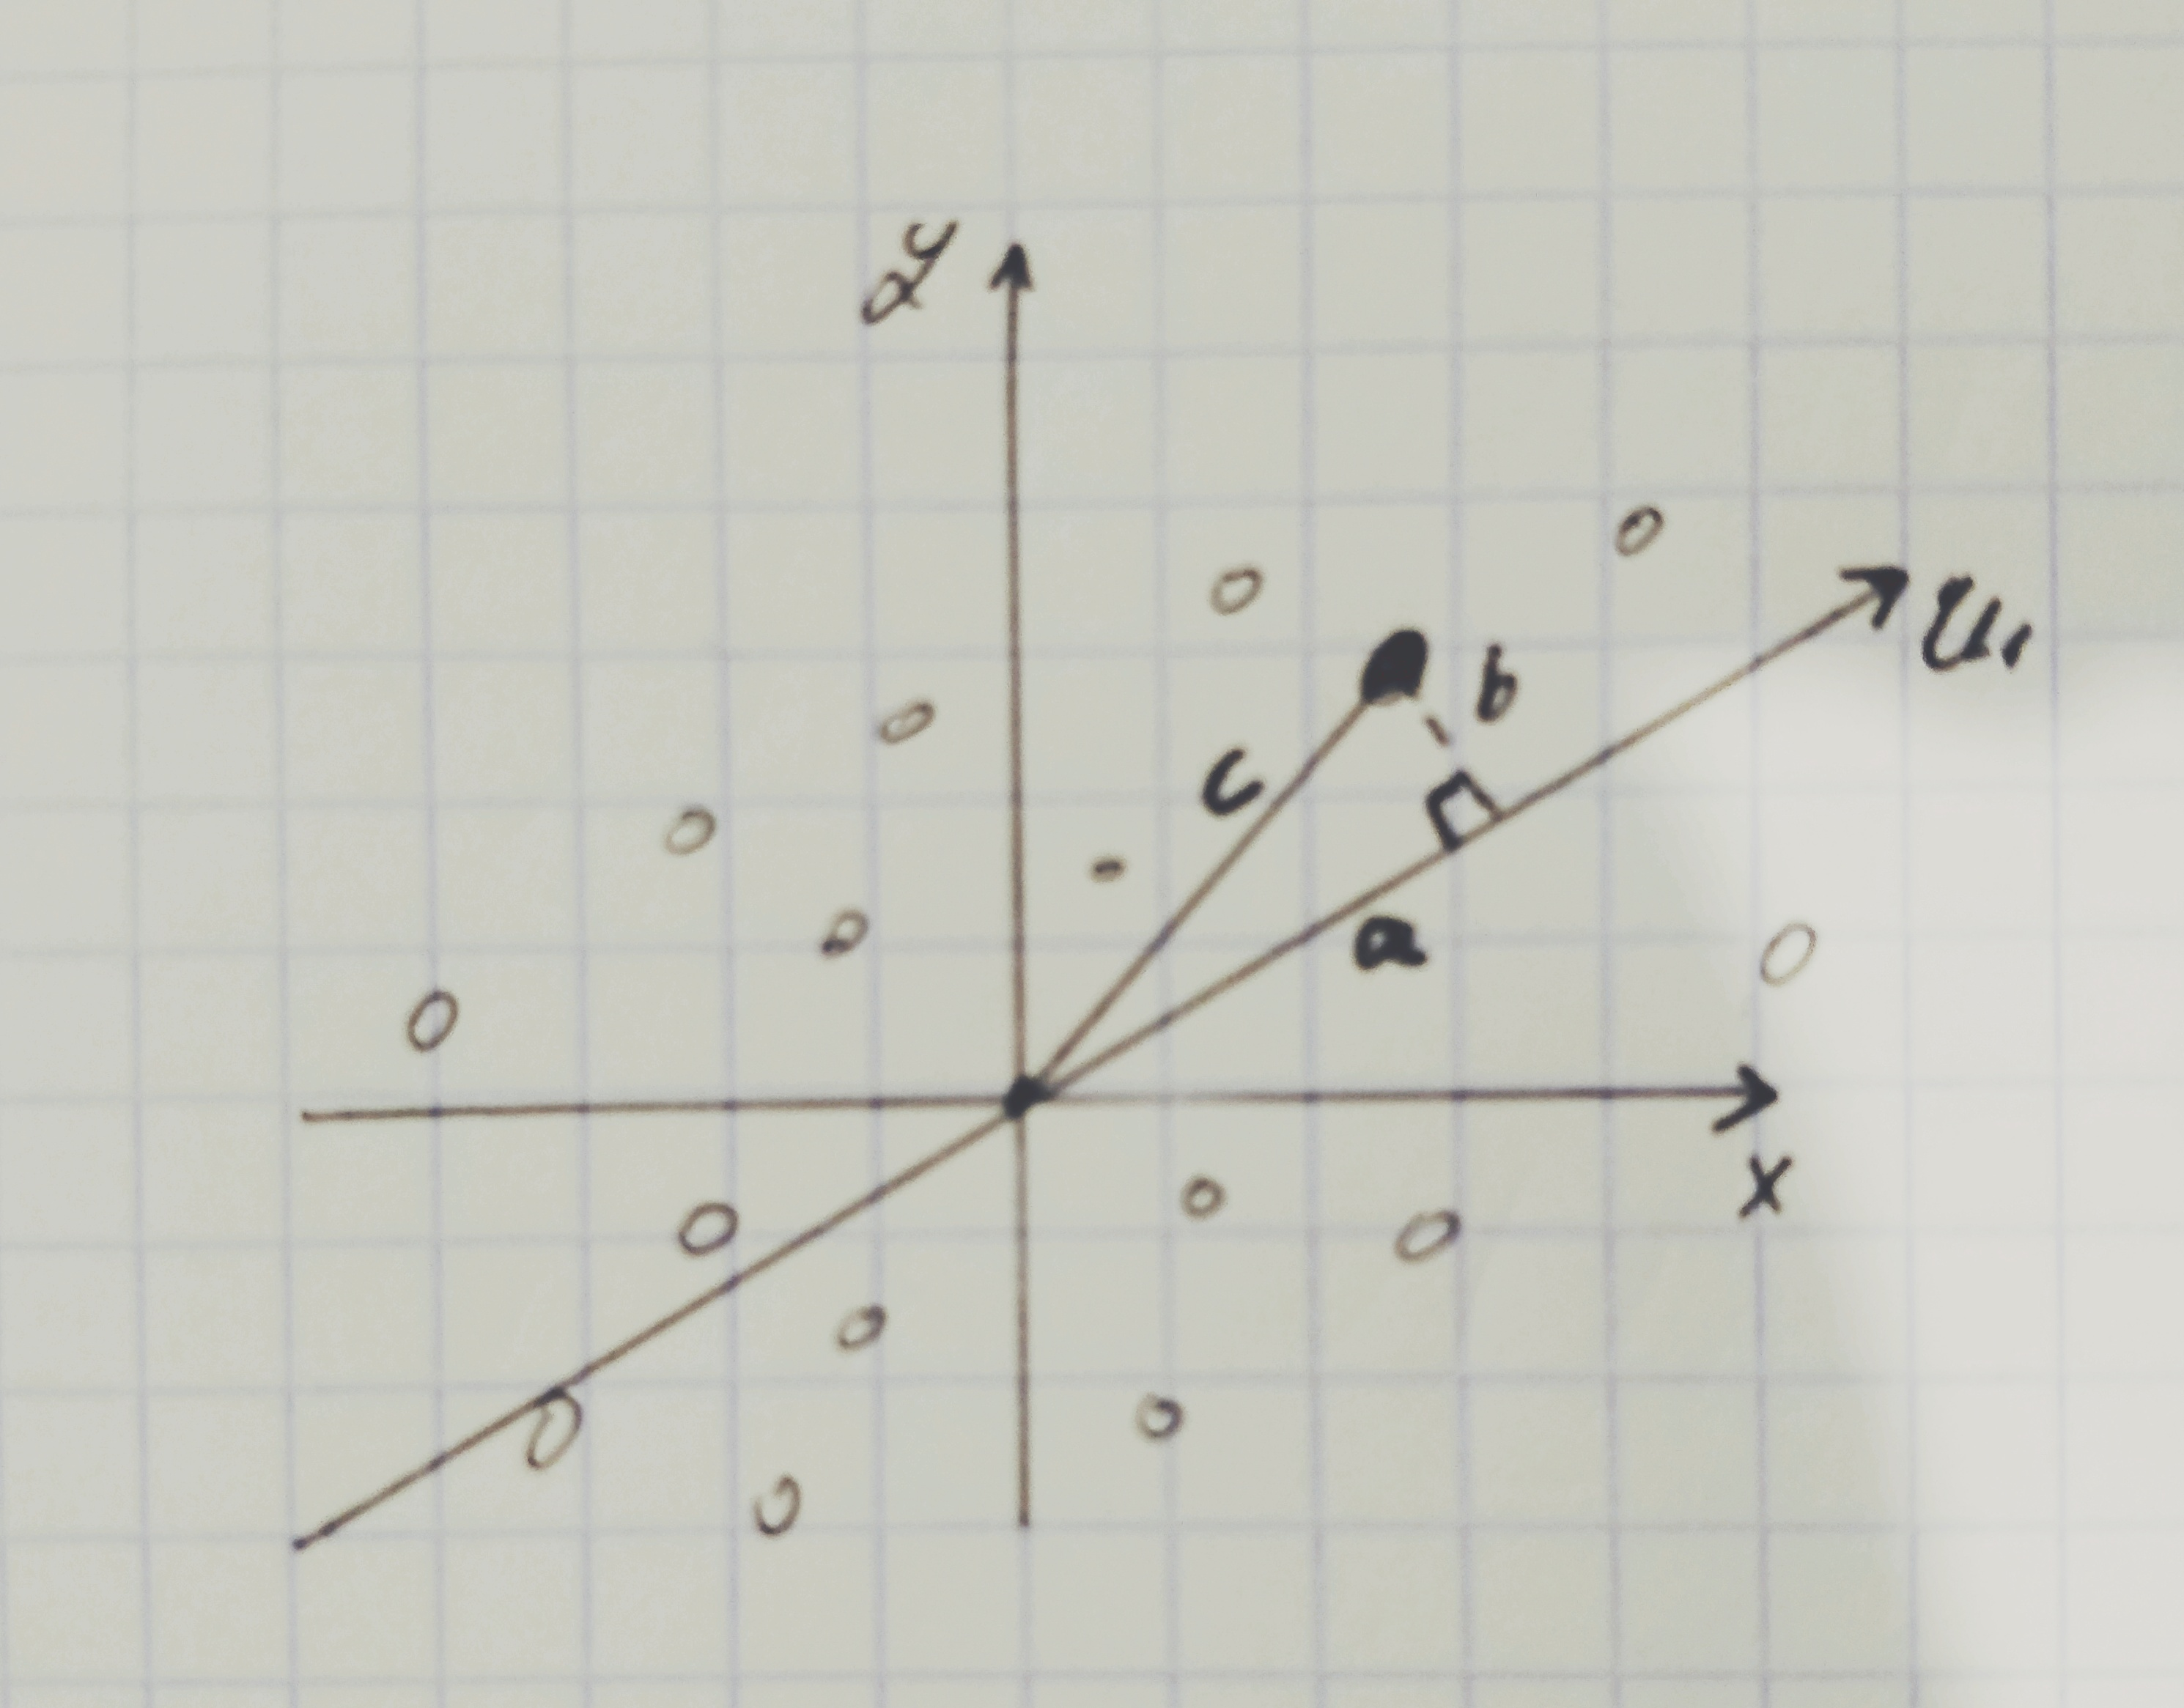
\includegraphics[width=0.5\textwidth]{chapters/unsupervised.learning/figures/7.1.jpg}
	\caption{\textbf{Link Between PCA Interpretations}: Projection of $\x_i$ onto $\vv{u}_1$ forming a right-angle triangle.}\label{pca_interp_link}
\end{figure}

\subsubsection{Projection- vs. Coordinates of Data-Points}
When considering PCA (or many other dimensionality reduction algorithms), an important but often overlooked point is the difference between projection and embedding (i.e coordinates) of the data-points. Suppose $\X\in\R^{m\times d}$ and we run the PCA algorithm to find a lower $k$ dimensional linear subspace. The optimal PCA solution is the subspace that minimizes the sum of squared distances between each data-point $\x_i$ and its orthogonal projection onto the subspace. As we have seen above (\ref{pca_closest_subspace}, \ref{pca_max_var}), this subspace is spanned by the $k$ leading eigenvectors of the $d\times d$ sample covariance matrix $S=\frac{1}{m}\sum\left(\x_i-\overline{x}\right)\left(\x_i-\overline{x}\right)^\top$.

~\\This matrix $U\in\R^{d\times k}$ enables the \textbf{projection} of the points in $\R^d$ onto the $k$ dimensional subspace, spanned by these leading eigenvectors. However, we would also like to actually reduce the dimension. Namely, find the map $W:\R^d\rightarrow\R^k$ and work with the dimension-reduced dataset $W\left(\x_1\right),\ldots,W\left(\w_m\right)$. As proven above, it is in fact $W=U^\top$ the map that provides the \textbf{embedding} of the data into the low dimension space. The vector $U^\top \x_i$ is a $k$ dimensional vector, laying within the found $k$ dimensional subspace. These are the \textbf{coordinates} of the original vector $\x_i$ according to the orthonormal set of $k$ leading eigenvalues of $S$.

~\\Let $\vv{u}_1,\ldots, \vv{u}_d$ be the $d$ eigenvectors of $S$ numbered in ascending order by the associated eigenvalues. As these vectors form a basis in $\R^d$, the vector $\x_i$ can be decomposed as $\x_i = \sum_{j=1}^d \inprod{\x_i}{\vv{u}_j}\vv{u}_j$. 
\begin{itemize}
	\item The \textbf{projecting} of $\x_i$ on the optimal $k$-dimensional subspace is given by $\x_i=\sum_{j=1}^k \inprod{\x_i}{\vv{u}_j}\vv{u}_j$.
	\item The \textbf{coordinates} (i.e. embedding) of $\x_i$ according to the $k$ leading principal vectors are given by: $\left(\inprod{\x_i}{\vv{u}_1},\ldots,\inprod{\x_i}{\vv{u}_k}\right)^\top$.
\end{itemize}

~\\In \autoref{pca_circ} we illustrate the difference between the projection and the coordinates (embedding) of the data-points. This dataset was generated as follows: 1000 points were sampled from the $\ell_2$ unit ball in $\R^2$. That is, $\left\{\left(\left(x_i\right)_1, \left(x_i\right)_2\right)\right\}^{1000}_{i=1}$ where $\left(x_i\right)_1^2+\left(x_i\right)_2^2=1$. Then Gaussian noise was added in a third axis: $$\left\{\left(\left(x_i\right)_1, \left(x_i\right)_2, \eps_i\right)\right\}^{1000}_{i=1} \quad \left(x_i\right)_1^2+\left(x_i\right)_2^2=1 \quad \eps_1,\ldots,\eps_{1000}\iid\Nc\left(0, 0.1\right)$$

~\\ \autoref{pca_circ} (left) shows this dataset. Then, using PCA we first project the data onto the subspace defined by the 3 PCs (\autoref{pca_circ}, center). At this point each data-point is still represented in $\R^3$, but we can indeed see that it is mainly the first 2 axes that capture the signal in the data, with the third axis showing only minor variations (the added noise). Lastly, when embedding the data into a 2 dimensional subspace (\autoref{pca_circ}, right), we are left with the true signal of the data (i.e. samples drawn from a 2 dimensional $\ell_2$ unit ball), and data-points are represented using only 2 coordinates.


\begin{figure}[!h]
	\centering
	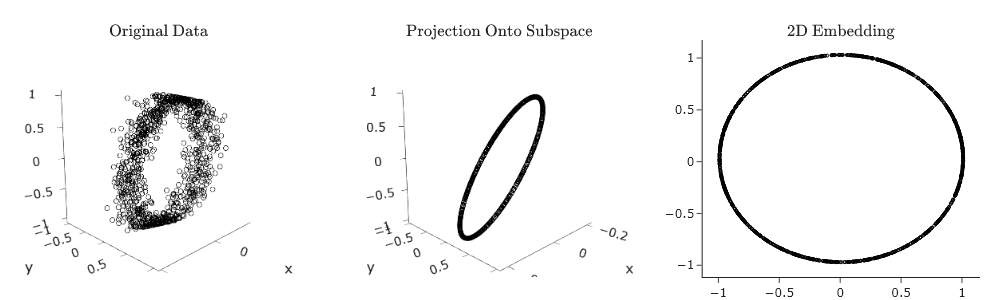
\includegraphics[width=0.9\textwidth]{chapters/unsupervised.learning/figures/pca_circ.png}
	\caption{\textbf{Projection vs. Embedding}: Dataset of sampels taken on the $\ell_2$ unit ball with Gaussian noise in $\R^3$, and then rotated in a random direction. \GitChapterSevelExamplesPCA}\label{pca_circ}
\end{figure}


\subsubsection{Principal Components As ``Typical Data-Points``}
The principal components found by PCA are vectors in the ambient space $\R^d$. This means that they share the same dimension as the data-points $\x_1,\ldots, \x_m$. As they are orthonormal vectors chosen such that the first $k$ provide the best linear approximation of dimension $k$ to the dataset, we can look at them in an interesting way. They are, in this sense, the ``typical`` data-points, maximally different from each other (as they are an orthonormal set). Thus, it is often interesting to see what they represent as data-points: what part of the ``signal`` do they capture.

~\\Returning to the MNIST Digits dataset of \autoref{pca_data_example} we can look at each principal component as a $28$-by-$28$ image. Then, we can think of the representation of each image by the linear combination of these images:

$$ \widehat{f}\left(\x\right) = \sum_{i=1}^k \alpha_i \vv{u}_i + \overline{\x}, \quad \alpha_1,\ldots,\alpha_k\in\R $$
where $\vv{u}_1,\ldots,\vv{u}_k$ are the leading $k$ principal components and $\widehat{\x}$ is the centering vector of the data. Notice that as this is a linear combination we are reconstructing the sample $\x$ via adding and subtracting (weighted) principal components.

\begin{figure}[h!]
	\centering
	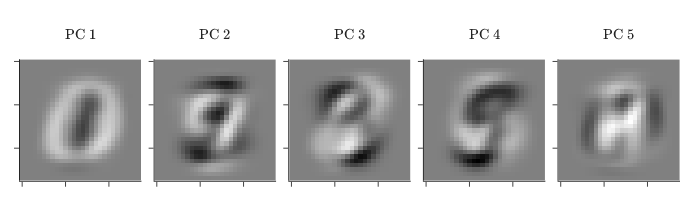
\includegraphics[width=0.9\textwidth]{chapters/unsupervised.learning/figures/pca_pcs_Digit.png}
	\caption{\textbf{Top Principal Components} of PCA fitted over the MNIST Digits dataset. \GitChapterSevelExamplesPCA}\label{pca_pcs}
\end{figure}

\autoref{anim:pca} shows the reconstruction process of an image of digit $4$ as the linear combination of the principal components. In each frame of the animation the restored image (center) is calculated as the restored image of the previous iteration plus $\alpha_i \vv{u}_i$ for $\vv{u}_i$ the principal component of the current iteration and $\alpha_i$ the loadings (coordinates) of the image for the $i$'th principal component.

\begin{figure}[h!]
	\centering
	\animategraphics[loop,autoplay,width=0.8\textwidth]{1}{chapters/unsupervised.learning/figures/pca_reconstruction_Digit-}{0}{25}
	\caption{\textbf{PCA Reconstruction:} Constructing image from principal components. \GitChapterSevelExamplesPCA}
	\label{anim:pca}
\end{figure}



\subsection{Kernel PCA}\label{kernel_pca}
The PCA algorithm discussed above is sometimes referred to as a ``Vanilla`` PCA, with many different variations of the algorithm to fit different scenarios. For one such variation, we apply kernel substitution techniques to obtain a \textbf{non-linear generalization} of PCA known as Kernel PCA (Sch\"olkopf \textit{et al.,} 1998). 
\\~\\Recall the general setup of Kernel methods: Suppose some algorithm $\Ac$ and let $\X\subset\Xc$ be an $m$-by-$d$ design matrix. For some mapping function $\phi:\Xc\rightarrow\mathcal{F}$, we first apply $\phi\left(\X\right)\coloneqq\left\{\phi\left(\x\right) | \x\in\X\right\}$ and then run $\Ac$ over $\phi\left(\X\right)$. By selecting $\phi$ is a smart manner we might be able to achieve a mapping to:
~\\\begin{itemize}
	\item A more informative feature space, where our algorithm will perform better (recall the use in Soft-SVM for non-separable datases \todo{add reference}).\\
	\item A new feature space of a much higher dimension (perhaps even of infinite dimension) while still being able to efficiently compute the transformation (i.e. $\phi$ a valid kernel function and use of the Kernel Trick).
\end{itemize}

~\\To apply the Kernel Trick on an algorithm $\Ac$ we require the algorithm to never access the data $\x\in\X$ directly, but only though the use of inner-products. Thus, in order to efficiently perform such kernel transformation and achieve a Kernel PCA algorithm, we must first show that we can re-write PCA to access the data only though inner-products.

\begin{claim}
Let $\X$ be a $m$-by-$d$ centered design matrix. Solving the PCA eigenvalue problem for $A=\X^\top\X$ is equivalent to solving the eigenvalue problem for $K=\X\X^\top$.
\end{claim}
\begin{proof}

In PCA we solve the eigenvalue problem of the matrix $A=\X^\top\X=\sum\x_i\x_i^\top$. We would like to represent this sum of outer-products via inner-products. Let $v$ be an eigenvector of $A$ corresponding eigenvalue $\lambda$ then: $$ \begin{array}{c} \lambda v = Av = \sum \x_i\x_i^\top v = \sum \inprod{\x_i}{v}\x_i \\ \Downarrow \\ v = \sum \frac{1}{\lambda} \inprod{\x_i}{v}x_i \end{array} $$

This means that solving an eigenvalue problem for $A$ is equivalent to finding a vector $v$ such that $$ \lambda\inprod{\x_i}{v} = \inprod{\x_i}{Av}\quad i=1,\ldots,m$$
Fix $i\in\left[m\right]$ and denote $\alpha_i = \frac{1}{\lambda}\inprod{\x_i}{v}$, so:
\begin{align}
\begin{array}{lcl}
\lambda\inprod{\x_i}{\sum_j \alpha_j\x_j} & = & \inprod{\x_i}{A\left(\sum_j \alpha_j\x_j\right)}\\
& = & \\
& = & \sum_j \alpha_j \inprod{\x_i}{A\x_j}\\
& = & \sum_j \alpha_j \inprod{\x_i}{\sum_l \x_l\x_l^\top \x_j}\\
& = & \sum_j \alpha_j \sum_l\inprod{\x_l}{\x_j}\x_l\\
& = & \sum_j \alpha_j \sum_l \inprod{\x_l}{\x_j}\inprod{\x_i}{\x_l}\\
& \Downarrow &\\
\lambda\sum_j \alpha_j\inprod{\x_i}{\x_j} & = & \sum_j \alpha_j \sum_l \inprod{\x_l}{\x_j}\inprod{\x_i}{\x_l} \label{eqn:kernel_pca_1}
\end{array}
\end{align}

Which in matrix notation is $\lambda K \alpha = K^2 \alpha$ where we define $K$ to be the Gram matrix over $\x_1,\ldots,\x_m$: $K_{ij} = \x_i^\top\x_j$, or equivalently $K=\X\X^\top$. For eigenvectors of $K$, not corresponding to zero eigenvalues the solution of $\lambda K \alpha = K^2 \alpha$ is equivalent to that of $\lambda \alpha = K \alpha$.
\end{proof}

Using the above claim, once we find $\alpha^{\left(1\right)},\ldots,\alpha^{\left(m\right)}$ the eigenvectors of $K$ we can then:
\begin{itemize}
	\item Obtain the eigenvectors of $A$ by $ v^{\left(l\right)}=\sum_{i=1}^m \alpha_i^{\left(l\right)}\x_i $.
	\item Project the data-points on the low dimension subspace by: 
	\begin{equation}
	\widetilde{\x}_l \coloneqq \inprod{v^{\left(l\right)}}{\x} = \sum_i \alpha^{\left(l\right)}\inprod{\x_i}{\x}
	\label{eqn:kernel_pca_2}
	\end{equation}
\end{itemize}

~\\Notice that by showingg that we can calculate the eigenvalues \ref{eqn:kernel_pca_1} and the projection \ref{eqn:kernel_pca_2} using the data only though inner-products we have shown that the Kernel Trick is applicable for the PCA algorithm. Thus, for a kernel function $\phi$ where $A=\sum\phi\left(\x_i\right)\phi\left(\x_i\right)^\top$:
~\\\begin{itemize}
	\item Solve the eigenvalue problem $\lambda\alpha = K\alpha$, for $K_{ij} = \inprod{\phi\left(x_i\right)}{\phi\left(\x_i\right)}$.
	\item Project the data-points by: $$	\widetilde{\x}_l \coloneqq \inprod{v^{\left(l\right)}}{\phi\left(\x\right)} = \sum_i \alpha^{\left(l\right)}\inprod{\phi\left(\x_i\right)}{\phi\left(\x\right)} = \sum_i \alpha^{\left(l\right)} k\left(\x_i,\x\right) $$
\end{itemize}

The above claim assumes the given design matrix $\X$ is centered. Unlike PCA, we cannot compute the mean and reduce it as it would require to compute $\phi\left(\X\right)$. Therefore, we would need to use a different approach:

\begin{lemma}\label{kernel_pca_centering}
Let $K$ be the Gram matrix of $\phi$ over the dataset $\X$. The centered Gram matrix to be used in the Kernel PCA algorithm is given by: $$ \widetilde{K} = K -\vv{1}_m K - K \vv{1}_m + \vv{1}_m K \vv{1}_m$$
\end{lemma}
\begin{proof}
Denote $\widetilde{\phi}\left(\x\right)$ the projected data-point after centerlizing: $$ \widetilde{\phi}\left(\x\right)=\phi\left(\x\right)-\frac{1}{m}\sum_l \phi\left(\x_l\right) $$ where $\vv{1}_m\in\R^{m\times m},\,\,\left[\vv{1}_m\right]_{ij} = 1/m$.
So the elements of the centered Gram matrix are given by:
$$
\begin{array}{ccl}
\widetilde{K}_{ij} & = & \inprod{\widetilde{\phi}\left(\x_i\right)}{\widetilde{\phi}\left(\x-j\right)} \\
& = & \inprod{\phi\left(\x_i\right)-\frac{1}{m}\sum_l \phi\left(\x_l\right)}{\phi\left(\x_j\right)-\frac{1}{m}\sum_k \phi\left(\x_k\right)}\\
& = & \phi\left(\x_i\right)^\top\phi\left(\x_j\right) -\frac{1}{m}\sum_k\phi\left(\x_i\right)^\top\phi\left(\x_k\right) -\frac{1}{m}\sum_l\phi\left(\x_l\right)^\top\phi\left(\x_j\right) + \frac{1}{m^2}\sum_{l,k}\phi\left(\x_l\right)^\top\phi\left(\x_k\right)\\
& = & K_{ij} - \frac{1}{m}\sum_l K_{il} - \frac{1}{m^2}\sum_k K_{jk} + \frac{1}{m}\sum_{l,k}K_{lk}
\end{array}
$$
which in matrix notation is $\widetilde{\phi}\left(\x\right)=\phi\left(\x\right)-\frac{1}{m}\sum_l \phi\left(\x_l\right)$.
\end{proof}

~\\So a pseudo-code for the Kernel PCA algorithm is:

\begin{algorithm}
	\caption{Kernel-PCA}\label{_kernel_pca_pseudo}
	\begin{algorithmic}
		\Procedure{Kernel-PCA}{$\X$, $k$, $l$}\Comment{$k$ the kernel computing $\phi$ and $l$ the dimension to reduce to}
		\State Compute the centered Gram matrix (\ref{kernel_pca_centering}): $$ \widetilde{K} = K -\vv{1}_m K - K \vv{1}_m + \vv{1}_m K \vv{1}_m,\quad K_{ij}\coloneqq k\left(\x_i,\x_j\right) $$
		\State Let $\alpha^{\left(1\right)},\ldots,\alpha^{\left(l\right)}$ be the eigenvectors of $\widetilde{K}$ corresponding the largest eigenvalues.
		\State Compute the corresponding eigenvectors of $A$ by: $\vv{v}^{\left(j\right)}\coloneqq\sum_{i=1}^m \alpha_i^{\left(j\right)}\x_i$
		\State \textbf{return} $\vv{v}^{\left(1\right)},\ldots,\vv{v}^{\left(l\right)}$
		\EndProcedure
	\end{algorithmic}
\end{algorithm}
~\\
\begin{remark}
The PCA algorithm seen in \autoref{pca_pseudo} diagonalizes the sample covariance matrix, which is a $d$-by-$d$ matrix and has a time complexity of $\mathcal{O}\left(d^3\right)$. If $d\gg m$ this can be computationally expensive. Though the proof of the Kernel PCA algorithm we have actually shown that we can solve the ``normal`` PCA by computing $\X\X^\top$ instead of using $\X^\top\X$. This means that time complexity is reduced to $\mathcal{O}\left(m^3\right)$ for computing $\X\X^\top$ and then $\mathcal{O}\left(m^2\cdot d\right)$ for adjusting the eigenvalues of $\X\X^\top$ to those of $\X^\top\X$. So we can update the PCA pseudo code as follows:\\

\begin{algorithm}
	\caption{PCA}\label{pca_pseudo2}
	\begin{algorithmic}
		\Procedure{PCA}{$\X$, $k$}\Comment{$\X$ The design matrix of $m$ samples and $d$ features}
		\If{$m>d$}
			\State Compute $A\gets \sum_{i=1}^m \left(\x_i-\overline{\x}\right)\left(\x_i-\overline{\x}\right)^\top$ 
			\State Let $\vv{u}_1,\ldots,\vv{u}_k$ be the eigenvectors of $A$ corresponding the largest eigenvalues.
			\State \textbf{return} $\vv{u}_1,\ldots,\vv{u}_k$
		\Else
			\State Compute $B\gets \X\X^\top$ \todo{write in format as of $A$}
			\State Let $\vv{v}_1,\ldots,\vv{v}_k$ be the eigenvectors of $B$ corresponding the largest eigenvalues.
			\State Compute the eigenvectors of $A$ by: $\vv{u}_i=\frac{1}{\norm{\X^\top\vv{v}_i}\X^\top\vv{v}_i}\quad i=1,\ldots,k$
			\State \textbf{return} $\vv{v}_1,\ldots,\vv{v}_k$
		\EndIf
		\EndProcedure
	\end{algorithmic}
\end{algorithm}
\end{remark}

\todo {Add exercise 12.26 in Bishop to explain why could remove $K$}



\section{Clustering}
A very useful set of learning problems is of clustering. Often, either as part of data exploration or as part of the main analysis, we are interested in partitioning our data into \textbf{meaningful} groups. For example, given a corpus of images we might want to divide them into different groups such as nature/urban/people/etc. photographs; or, given the set of genes in the human genome, we might want to group together genes associated with specific diseases. In both these examples we are only given the samples (images or genes) but we do not have any \textbf{ground truth} (labels). We are not given the information of what is seen in each image, nor for each disease what genes are associated with it. 

~\\We would therefore want to define some measure of \textit{similarity} between samples of a given domain. Using this similarity we could split the data into different subsets, where intuitively samples within a given set are \textit{more similar} to one another compared to samples of different sets.

\begin{remark}
This form of clustering, where we partition the data into distinct non-overlapping groups is also referred to as ``hard assignment`` as each sample is assigned to one specific subset. Sometimes, rather than assigning to some specific cluster we are interested in ``partly assigning`` to multiple clusters. This is referred to as ``soft assignment/clustering``.
\end{remark}

\subsection{K-Means}
Though there are many different approaches to perform clustering, common to many is the notion of defining some representative data-point of the cluster. Then, clustering of data-points give the given sample is perform with respect to these cluster representatives.

\begin{definition}
A partition of a dataset $\left\{\x_i\right\}_{i=1}^m$ is a set $C_1,\ldots,C_k$ such that $\left\{\x_i\right\}_{i=1}^m = \biguplus_{j=1}^k C_j$
\end{definition}

Given some partition over the data and the representative data-points, we can define a \textbf{cost function} for the partition. For some metric (i.e. distance function) over the data $d:\Xc\times\Xc\rightarrow \R_+$ we define:
\begin{equation}
G_d\left(C_1,\ldots,C_k, \mu_1,\ldots,\mu_k\right) \coloneqq \sum_{j=1}^k \sum_{\x\in C_j} d\left(\x,\mu_j\right)
\end{equation}
where $\mu_1,\ldots,\mu_k$ are the representatives of clusters $C_1,\ldots,C_k$. Using this function, the goal is to find the partitioning that minimizes the following:
\begin{equation}
\left\{C_1,\ldots,C_k\right\}^* = \underset{\left\{C_j,\mu_j\right\}_{j=1}^k}{argmin} G_d\left(C_1,\ldots,C_k,\mu_1,\mu_k\right) = \underset{\left\{C_j,\mu_j\right\}_{j=1}^k}{argmin} \sum_{j=1}^k \sum_{\x\in C_j} d\left(\x,\mu_j\right)
\label{eqn:cluster_cost}
\end{equation}

~\\In the case of the $k$-means algorithm the cluster representatives are chosen to be: $$ \mu_j\left(C_j\right) \coloneqq \underset{\mu\in\Xc}{argmin}\sum_{\x\in C_j} d\left(\x,\mu\right)  $$

In order to find the minimizers of \ref{eqn:cluster_cost} we would have to navigate the space of all possible partitions of $m$ objects into $k$ subsets. As there are an exponential amount of such subsets, minimizing the cost function $G$ is NP-hard, and we must resort to \textbf{heuristics}. The most famous heuristic for minimizing $G$, when $d$ is the Euclidean distance, is k-means.

\begin{algorithm}
	\caption{K-Means}\label{kmeans_pseudo}
	\begin{algorithmic}
		\Procedure{K-Means}{$\X$, $k$}\Comment{$\X$ The design matrix of $m$ samples and $d$ features}
		\State Choose initial centroids $\mu_1,\ldots,\mu_k$ randomly.
		\While{Not converged}
			\State \textbf{Assignment:} Assign each point $\x_i$ to the centroid closest to it: $$ C_j^{\left(t\right)}\coloneqq \left\{\x | \mu_j = argmin_{\mu}\,\,d\left(\x,\mu\right),\x\in\X\right\} $$
			\State \textbf{Update}: Adjust cluster centroids by: $ \forall j\in\left[k\right] \quad \mu_j^{\left(t+1\right)} \coloneqq \left|C_j^{\left(t\right)}\right|^{-1}\sum_{\x\in C_j^{\left(t\right)}}\x $
		\EndWhile
		\State \textbf{return} $C_1,\ldots,C_k$
		\EndProcedure
	\end{algorithmic}
\end{algorithm}


~\\ This clustering approach uses \textbf{Lloyd's Algorithm} to minimize $G$ using an iterative strategy where each time we \textbf{alternate} between minimizing two terms. We first define a partition of the dataset, associating points to subsets by their nearest centroid. These subsets are called Voronoi cells. Then we re-calculate the cluster's centroid.


\begin{figure}[h!]
	\centering
	\animategraphics[loop,autoplay,width=0.45\textwidth]{1}{chapters/unsupervised.learning/figures/kmeans-basic-}{0}{14}
	%	\caption{\textbf{Polynomial Fitting:} Fitted polynomial of degree $1$ over different datasets differing only in values of added sample noise. \todo{reference to github code}}
	\label{anim:kmeans1}
\end{figure}

\subsubsection{Convergence to Multiple- and Sub- Optimal Solutions}
As clustering problems are NP-Hard, the K-Means algorithm algorithm uses the Lloyd's algorithm heuristic to find a good partition of the data. Being a heuristic, the optimality of the algorithm assignment to clusters isn't guaranteed. In fact, due to the nature of the random initialization of centroids, the K-Means algorithm might converge into a sub-optimal solution or to there exists more than a single possible optimal solution.~\\

Sub-optimality means that given a dataset $\left\{\x_i\right\}^m_{i=1}$ the K-Means algorithm returned some partitioning $C_1,\ldots,C_k$ such that there exists a different partitioning of the data $C_1',\ldots,C_k'$ with a lower objective value: $G\left(C_1,\ldots,C_k\right) > G\left(C_1',\ldots,C_k'\right)$. This is the product of the objective function not being convex, which means there could be several local minima, each achieving a different cost. In \autoref{anim:kmeans2} we see 4 groups of data-points and two initial centroids, positioned in such a way that forces the algorithm to converge into a sub-optimal solution. Optimal assignment is achieved for final centroids $\mu_i=\left(0,5\right), \mu_j=\left(20,5\right),\,\,i\neq j$.

\begin{figure}[h!]
	\centering
	\animategraphics[loop,autoplay,width=0.45\textwidth]{1}{chapters/unsupervised.learning/figures/kmeans-suboptimal-}{0}{4}
	\caption{\textbf{Suboptimal Solution:} Data-points and initial centroids leading to a suboptimal solution.}
	\label{anim:kmeans2}
\end{figure}



Multiple optimal solution means that given a dataset $\left\{\x_i\right\}^m_{i=1}$ there are more than a single possible partitioning of the data that will yield the lowest objective value. It is important to note, that whenever discussing clustering assignments, we always look at the partitioning up to a permutation of the partition names. That is, suppose we are given the samples $1,2,3,4,5$ the partitioning of $C_1=\left\{1,2,3\right\},C_2=\left\{4,5\right\}$ is identical to $C_1=\left\{4,5\right\},C_2=\left\{1,2,3\right\}$, and clearly, both will achieve the same objective value. When referring to multiple optimal solution we mean:
$$
\begin{array}{ll}
Given \,\,\left\{\x_i\right\}^m_{i=1}  & \exists\left\{C_1\ldots,C_k\right\},\left\{C_1',\ldots,C_k'\right\} \\
For \,\, which & G\left(C_1,\ldots,C_k\right) = G\left(C_1',\ldots,C_k'\right)\\
It \,\, holds \,\, that & \exists j\in\left[k\right] \,\,\,\forall l\in\left[k\right]\quad C_j\neq C_l'
\end{array}
$$
and that they achieve an objective value lower (or equal) to any other partitioning of the dataset. An example for such dataset and initialization of centroids is seen in \autoref{anim:kmeans2}. In this case both centroids are initialized in the center of all data points.

\begin{figure}[h!]
	\centering
	\animategraphics[loop,autoplay,width=0.4\textwidth]{1.07}{chapters/unsupervised.learning/figures/kmeans-multiple-a-}{0}{8}
	\animategraphics[loop,autoplay,width=0.4\textwidth]{1}{chapters/unsupervised.learning/figures/kmeans-multiple-b-}{0}{6}
	\caption{\textbf{Multiple Optimal Solutions:} Data-points and initial centroids leading to two different optimal solutions}
	\label{anim:kmeans3}
\end{figure}



\subsubsection{Selection of $k$}
As in different algorithms previously seen, in K-Means too we are required to provide a value for the hyper-parameter $k$. As we do not know how many clusters we really have in the dataset this is not a simple task. Notice that as long as we have more data-points than clusters, for any optimal solution with $k$ clusters, we can achieve a solution with a lower objective for $k+1$. As such, simply running over different values of $k$ and selecting the minimal value isn't a viable solution. Instead, we will apply a similar technique to the one used in PCA. We will plot the to objective achieved for different values of $k$ and select the value after which the improvement is less drastic. In \autoref{selecting-k} we apply this strategy over the dataset seen in \autoref{anim:kmeans1}. As seen in the elbow-plot once we reach $k=4$, the incremental improvement in score is much lower. Since the data was generated from 4 different Gaussians, this approach managed to find the correct value.
	
\begin{figure}[!h]
	\centering
	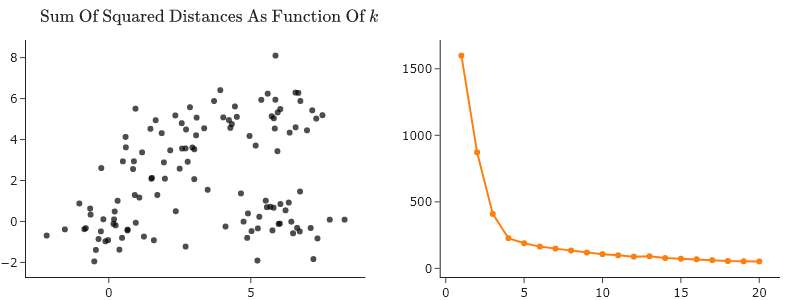
\includegraphics[width=0.6\textwidth]{chapters/unsupervised.learning/figures/kmeans-selecting-k.png}
	\caption{\textbf{Selecting $k$ hyper-parameter in K-Means}}\label{selecting-k}
\end{figure}
